\chapter{Sparse Field - Implemented code}
\label{implementedChap}
\section{Introduction}
The sparse field level set method was implemented in C++ for the project, and the implemented code is mainly based on the pseudocode in \cite{lankton09}, which again is based on Whitaker's introduction to the sparse field method in \cite{whitaker89}. 
The sparse field was first implemented in 2D and after bugfixing and some test-runs it was extended to 3D, which executes and runs in the exact same way as the 2D version. The implemented code of the 2D and 3D versions the implemented code can be found in appendix A and B respectively. A parallelized verson of the 2D version was also implemented in CUDA, and the source code is found in Appendix C. This chapter will give a detailed explanation of the implemented code and how it works. Henceforth, when the word pixel is meantioned it can have slightly different meanings. Elements in different arrays will be referred to as pixels (even if they actually are integer of floating point values), as will the elements in all the lists. 

\section{The layers and their representation}
As previously mentioned, the sparse field method can be implemented using linked lists to hold the pixels being used in the calculations. These pixels are seperated into five layers, each represented by a linked list. One of the lists holds the active points, i.e the zero level set, and is referred to as the Lz list. The rest of the needed pixels are seperated according to their closeness to the pixels in Lz and on which side of the Lz pixels they are located. The Ln1 list contains the pixels that are adjacent to Lz pixels on the inside of the object being segmented. Similarly Lp1 contains pixels that are adjacent, but on the outside. All pixels that are adjacent to those in Ln1 except for those in Lz are elements in the Ln2 list, and similarly the ones adjacent to Lp1 on the opposite side of Lz are part of Lp2. This becomes more clear when looking at table \ref{rangeTab1} and figure \ref{labelExample}. The elements in these lists are C/C++ structures (struct) called $Pixel$ which contains two (three in 3D) integer values x and y representing its coordinates in $\phi$. So when an element in $\phi$ is to be added to a any of the layers, the coordinates in $\phi$ of that element is used to create a new $Pixel$ which is added to the list corresponding to the layer in question. 

\begin{table}[h] %h = here
	\centering
	\begin{tabular}{| c | c |} 
	% l = left-justified columns, alternatives are: r (right) and c (center)
	% | = vertical line, \hline = horizontal line
	\hline
	List Name & Range\\ 
	\hline
	Lz & $[-0.5, 0.5]$\\
	Ln1 & $[-1.5, -0.5\}$\\
	Lp1 & $[0.5, 1.5]$\\
	Ln2 & $[-2.5, -1.5\}$\\
	Lp2 & $\{1.5, 2.5]$\\
	\hline
	\end{tabular}
	\caption{Range of lists used in \cite{lankton09}}
	\label{rangeTab1}
\end{table}

\begin{figure}[h!]
\centering

\includegraphics[width=0.65\textwidth]{implemented/labelExample}
\caption{Label image: image showing the different layers under segmentation.}
\label{labelExample}
\end{figure}
Table \ref{rangeTab1} shows the ranges used by Whitaker in \cite{whitaker89} when describing the layers used in the sparse field method. Figure \ref{labelExample} represents the 5 different layers with different colors. The pixels in the zero level set are represented as dark-purple colored, Lp1 is represented by light purple and the outer-most (light-blue) pixels are members of Lp2. Ln2 is dark-blue and Ln1 is brown, and these two layers plus the dark part are defined to be inside the object being segmented at a given iteration. The two other layers and the white part is defined to be outside the object. This type of image will be referred to as the $label$ image/array, because it shows the label assigned to each pixel of the image being segmented.

By looking closer at table \ref{rangeTab1} it can be seen that Lz has a slightly wider range than the other lists. This range of exactly 1 does in some cases cause problems that lead to disortions and artifacts in the segmentation. What these problems are will be discussed in \ref{ProblemsMet}. To overcome these problems the ranges of the lists were slightly changed to make all the lists equal in range. The range-corrected lists used in the implementation are shown in table \ref{rangeTab2}, and even though the change seems small and insignificant it improves the result significantly (as will be discussed in \ref{ProblemsMet}).

\begin{table}[h] %h = here
	\centering
	\begin{tabular}{| c | c |} 
	% l = left-justified columns, alternatives are: r (right) and c (center)
	% | = vertical line, \hline = horizontal line
	\hline
	List name & Range\\
	\hline
	Lz & [-0.5, 0.5\}\\
	Ln1 & [-1.5, -0.5\}\\
	Lp1 & [0.5, 1.5\}\\
	Ln2 & [-2.5, -1.5\}\\
	Lp2 & [1.5, 2.5\}\\
	\hline
	\end{tabular}
	\caption{Range of lists used in the implementation}
	\label{rangeTab2}
\end{table}

\section{Datastructures and types used}
In addition to the five lists representing the five layers, two arrays of equal size and dimension as the image to be segmented are used. One of them is the $label$ image described above, which is used to track where the pixels containing the different layers are on the domain. Given a pixel, to find out which layer (if any) it is a member of, a simple lookup to the $label$ array is enough. Another excellent feature of the $label$ array is that it can be used to visually verify if all the layers are correclty aligned and if there are any pixels of any layer that are poorly placed. The $label$ image can thus be used to find artifacts that might have resulted from code errors by an user visually looking at it, which proved to be of excellent help when debugging. An example of a $label$ image which clearly states that there is something wrong with how the layers are handled in the code is shown in figure \ref{labelFailedEx} (zoomed in for clarity). How that $label$ image actually should have been is illustrated in figure \ref{labelOkEx}.

\begin{figure}[h!]
\centering
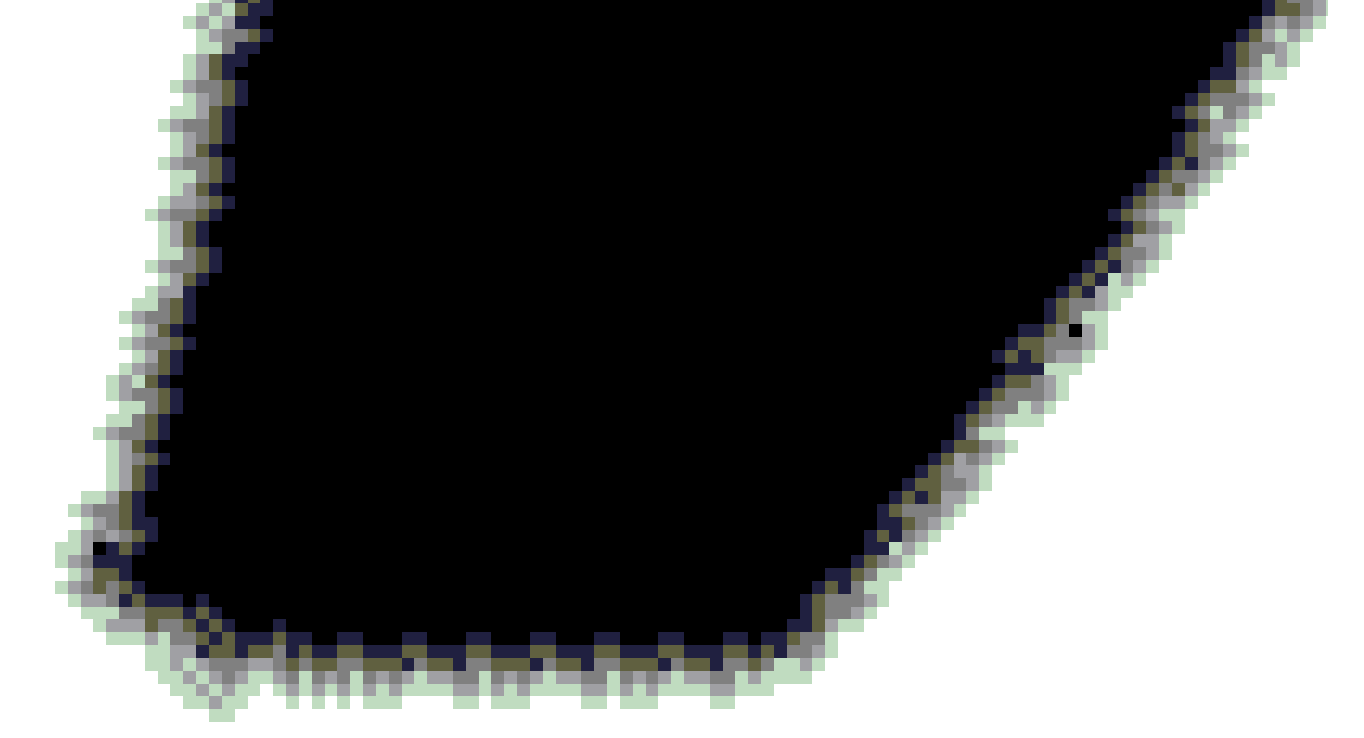
\includegraphics[width=0.90\textwidth]{implemented/labelFailedEx}
\caption{A label image with artifacts due to code errors when handling the layers.}
\label{labelFailedEx}
\end{figure}

\begin{figure}[h!]
\centering

\includegraphics[width=0.90\textwidth]{implemented/labelOkEx}
\caption{How the label image should have been.}
\label{labelOkEx}
\end{figure}

The other array used is the $\phi$ - array, which contains the actual $\phi$ values of each pixel in the domain. The range of the values is exactly the same as in the $label$ image, but while the $label$ image only contains integer values describing which layer a pixel is part of, the $\phi$ image contains the actual values (floating point numbers) of the level set. The images represented by the $label$ and $\phi$ arrays would thus be very similar (though small differences may be seen) when looking at, but they do have different tasks. The $label$ is as mentioned used as a lookup table, while the $\phi$ array determines which layer a pixel belongs to after its pixels have been updated with the speed function.

To correctly move pixels between the layers some temporary lists have to be used, one for each layer. By using these temporary lists, called Sn2, Sn1, Sz, Sp2 and Sp2, elements in the corresponding Ln2, Ln1, Lz, Lp1 and Lp2 lists are prevented from being moved more than once in a single iteration.

\section{Levelset evolution process}
First all pixels in Lz are updated by the speed function. Some (or all) of these pixels may at that point in time have values outside of Lz's range. The pixels in Lz with values smaller than -0.5 will then be removed from Lz and added to Sn1, while those with values greater than or equal to 0.5 will be removed from Lz and added to Sp1. This process is show in the pseudocode in algorithm \ref{SzAdd}.
\begin{algorithm}[h!]
\begin{algorithmic}[1] %[n] means numbering of the n'th lines, so [1] means numbering of each line
\ForAll{$p \in Lz$} \Comment{$p$ = Pixel}
	\State $\phi(p.x, p.y) = \phi(p.x, p.y) + speedFucntion(p.x, p.y)$ 
	\If{$\phi(p.x, p.y) \geq 0.5$}
		\State sp1.add(e)
		\State Lz.remove(e)
	\ElsIf{$phi(e.x, e.y) < -0.5$}
		\State Sn1.add(e)
		\State Lz.remove(e)
	\EndIf
\EndFor
\end{algorithmic}
\caption{Update elements in Lz with the speed function and transfer to Sp1 or Sn1.}
\label{SzAdd}
\end{algorithm}
This process of updating the pixels with new values and moving them to neighbouring lists if they are not within the range of the list is executed for all the other lists as well. The difference with Lz and the rest is that while the pixels in Lz are directly updated by the speed function while the pixels in the other lists are not. The definition of pixels in Ln1 and Lp1 say that they are neighbours of pixels in Lz, which makes a recomputation of the speedfunction for these pixels unnecessary. When Lz moves in one direction, Ln1 and Lp1 must move in the same direction, resulting in Ln2 and Lp2 doing the same. This process of following Lz can be accomplished in code by several means, but doing it as in the pseudocode in algorithm \ref{minMaxAndLn1} proved to give good results. For pixels in Ln2 and Ln1 the greatest value from a pixel's four neighbours (over, under, left, right, and pixels in front and back for 3D) in $label$ is found, and then that pixel is assigned the found value minus one. Similarly for Lp2 and Lp1 the smallest value of the neighbours is found, and the pixel is assigned that value plus one. In algorithm \ref{Ln12Update} Ln1 and Lp1 are updated similarly to Lz in algorithm \ref{SzAdd} using the algorithm in \ref{minMaxAndLn1} to update $\phi$. Algorithm \ref{Lp12Update} shows the same for Ln2 and Lp2. Notice that the $label$ arraysof the pixels moving out of Ln2 and Lp2 is updated in \ref{Lp12Update}. This is not the case in algorithm \ref{SzAdd} and \ref{Ln12Update} because the pixels of Ln1 and Lp1 are depended on the values of the $\phi$ and $label$ arrays of the pizel who are in Lz. Likewise, Lp2 and Ln2 are dependent on the values of Lp1 and Ln1. Also notice that pixels moving out of Ln2 (not those moving to Ln1, but the other direction) are having their corresponding values in the $\phi$ and $label$ arrays set to -3, and those moving out of Lp2 to 3.

\begin{algorithm}[h!]
\begin{algorithmic}[1]
\Procedure{follow}{$p, greaterOrLess, checkAgainst$} 
\Statex \Comment{$p$ = Pixel, $greaterOrLess, checkAgainst = integer$}
\State $result$ = $checkAgainst$
\If{$greaterOrLess = 1$} \Comment{true for: Ln1 or Ln2 pixles}
	\ForAll{$n \in N(p)$} 
		\Statex \Comment{$N(p)$ = neighbouring pixels: over, under, left, right}
	  	\If{label($n.x, n.y$) $>$ result}
	  		\State $result$ = $\phi(n.x, n.y)$
	  	\EndIf
	\EndFor
\EndIf
\If{$greaterOrLess = -1$}  \Comment{true for: Lp1 or Lp2 pixles}
 	\ForAll{$n \in N(p)$}
	  	\If{label($n.x, n.y$) $<$ $result$}
	  		\State $result$ = $\phi(n.x, n.y)$
	  	\EndIf
	\EndFor
\EndIf
\Return $result$
\EndProcedure
\end{algorithmic}
\caption{How Ln2, Ln1, Lp1, Lp2 follows after Lz.}
\label{minMaxAndLn1}
\end{algorithm}

\begin{algorithm}[h!]
\begin{algorithmic}[1] %[n] means numbering of the n'th lines, so [1] means numbering of each line
\ForAll{$p \in Ln1)$}
	\If{$p$ has no neighbour that is part of Lz}
		\State Sn2.add(p)
		\State Ln1.remove(p)
	\Else
		\State $M = follow(p, 1, 0)$ 
		\State $phi(p.x, p.y) = M-1$
		\If{$phi(p.x, p.y) \geq -0.5$}
			\State Sz.add(p)
			\State Ln1.remove(p)
		\ElsIf{$phi(p.x, p.y) < -1.5$}
			\State Sn2.add(p)
			\State Ln1.remove(p)
		\EndIf
	\EndIf
\EndFor

\ForAll{$p \in Lp1)$}
	\If{$p$ has no neighbour that is part of Lz}
		\State Sp2.add(p)
		\State Lp1.remove(p)
	\Else
		\State $M = follow(p, -1, 0)$ 
		\State $phi(p.x, p.y) = M+1$
		\If{$phi(p.x, p.y) < 0.5$}
			\State Sz.add(p)
			\State Lp1.remove(p)
		\ElsIf{$phi(p.x, p.y) \geq 1.5$}
			\State Sp2.add(p)
			\State Lp1.remove(p)
		\EndIf
	\EndIf
\EndFor
\end{algorithmic}
\caption{Update elements in Ln1 and Lp1}
\label{Ln12Update}
\end{algorithm}

\begin{algorithm}[h!]
\begin{algorithmic}[1] %[n] means numbering of the n'th lines, so [1] means numbering of each line
\ForAll{$p \in Ln2)$}
	\If{$p$ has no neighbour that is part of Ln1}
		\State $label(p.x, p.y) = -3$
		\State $phi(p.x, p.y) = -3$
		\State Ln2.remove(p)
	\Else
		\State $M = follow(p, 1, -1)$ 
		\State $phi(p.x, p.y) = M-1$
		\If{$phi(p.x, p.y) \geq -1.5$}
			\State Sn1.add(p)
			\State Ln2.remove(p)
		\ElsIf{$phi(p.x, p.y) < -2.5$}
			\State $label(p.x, p.y) = -3$
			\State $phi(p.x, p.y) = -3$
			\State Ln2.remove(p)
		\EndIf
	\EndIf
\EndFor

\ForAll{$p \in Lp2)$}
	\If{$p$ has no neighbour that is part of Lp1}
		\State $label(p.x, p.y) = 3$
		\State $phi(p.x, p.y) = 3$
		\State Lp2.remove(p)
	\Else
		\State $M = follow(p, -1, 1)$ 
		\State $phi(p.x, p.y) = M+1$
		\If{$phi(p.x, p.y) < 1.5$}
			\State Sp1.add(p)
			\State Lp2.remove(p)
		\ElsIf{$phi(p.x, p.y) \geq 2.5$}
			\State $label(p.x, p.y) = 3$
			\State $phi(p.x, p.y) = 3$
			\State Lp2.remove(p)
		\EndIf
	\EndIf
\EndFor
\end{algorithmic}
\caption{Update elements in Ln2 and Lp2.}
\label{Lp12Update}
\end{algorithm}

When all pixels moving from one layer to another layer have been adressed, pixels moving into Lp2 and Ln2 from the outside have to be added to Sp2 and Sn2. This is accomplished by simply adding all neighbours of Lp1 and Ln1 who are not part of any layer to Sp2 and Sn2 respectively, and update their value by incrementing or decrement by one to reflect the range of the lists they are moved to. How this actually is implemented can be seen in algorithm \ref{updateLevelSets}, which includes the updating of the lists by their corresponding temporary list. Alogrithms \ref{SzAdd}, \ref{Ln12Update}, \ref{Lp12Update} and \ref{updateLevelSets} (in that order) is the complete set of actions executed in each iteration of the segmentation process.

\begin{algorithm}[h!]
\begin{algorithmic}[1]
	\ForAll{$p \in Sz)$}
		\State $label(p.x, p.y) = 0$
		\State Lz.add(p)
	\EndFor
	\State Reset Sz
	
	\ForAll{$p \in Sn1)$}
		\State $label(p.x, p.y) = -1$
		\State Ln1.add(p)
		\ForAll{$n \in N(p)$} 
			\If{$phi(n.x, n.y) = -3$}
				\State Sn2.add(n)
			\EndIf
		\EndFor
	\EndFor
	\State Reset Sn1
	
	\ForAll{$e \in Sp1)$}
		\State $label(p.x, p.y) = 1$
		\State Lp1.add(p)
		\ForAll{$n \in N(e)$}
			\If{$phi(n.x, n.y) = 3$}
				\State Sp2.add(n)
			\EndIf
		\EndFor
	\EndFor
	\State Reset Sp1
	
	\ForAll{$p \in Sn2)$}
		\State $label(p.x, p.y) = -2$
		\State Ln2.add(p)
	\EndFor
	\State Reset Sn2
	
	\ForAll{$p \in Sp2)$}
		\State $label(p.x, p.y) = 2$
		\State Lp2.add(p)
	\EndFor
	\State Reset Sp2
\end{algorithmic}
\caption{Updating by using the temporary lists.}
\label{updateLevelSets}
\end{algorithm}
\clearpage

\subsection{Code structure - FIKS DETTE}
The code is seperated into two C++ files, main.cpp and update.cpp, and two corresponding header files. The update.cpp file consist of everything that happens at each iteration, this icnludes calculating the speed function, updating the $\phi$ - array with the speed, updating the $label$ array and update the lists. The main.cpp file consist of actions that are executed before and after the actual segmentation, such as initializing everything, handle input and reading/writing to/from the input image and segmentation result. 

\subsection{Input and initialization}
The program takes four inputs, the total number of iterations, threshold, epsilon and alpha. More inputs can be defined as input, e.g. seed points and the location of the input file, but these are currently set in the code because too many inputs is unnecessary when running the problem with a few different data sets. Handling of the input code is however set up in a way that makes adding more inputs a simple task. 

An array of same size as $label$ and the $\phi$ arrays is used to initialize $label$, the $\phi$ and Lz. This array, called init, is initialized to zero valued elements at start, and then filled with 1's given the x,y (and z in 3D) coordinates of the seed point(s). The seed point creates a circle (or sphere if 3D) of 1's in the init array that represents the starting position. Based on the values in init the two arrays $label$ and $\phi$ are initialized. All pixels in $label$ and $\phi$ corresponding with those in init with value 1 are set to -3 to indicate that they are inside the segmentation object. All other pixels in $label$ and $\phi$ are set to 3 indicating that they are outside the object. Then the corresponding pixels to all values in init that are 1 but have 0 valued neighbours are set to 0, indicating that they are part of the zero level set. Then these pixels are added to Lz as initial zero level set values. Then $Ln1$, $Lp1$, $Ln2$ and $Lp2$ are filled according to their definitions, and the $label$ and $\phi$ arrays are updated to refelct these changes. After these initializing actions are finished the segmentation process can start.

\subsection{Speed function explained}
Two different speed functions are implemented. These are seperatly implemented in their own methods, and a speed function is only referenced in one place in the code. This makes it easy to implement new speed functions, and to change between which of them to use when running the program. The speed function methods takes in as parameters the coordinates of the pixel to calculate the speed chnage on, and returns a value which then is added to the speed from the last iteration. The two speed functions are implemented are the ones explained in chapter \ref{levelSetChap}. The simplified Chan-Vese speed function was first implemented, and only used to test wether the rest of the implemented sparse field code worked as expected. Because this simple function behaves much like a region grow function it will not be a part of the discussion in the result chapter. 

The other speed function was implemented as explained in chapter \ref{levelSetChap}, except for some parts that were dropped because it was not needed in this verion of the sparse field. A short description of how the speed function is calculated is shown in algorithm \ref{implSpeedAlg}

\begin{algorithm}[h!]
\begin{algorithmic}[1]
\Procedure{speedFunction}{$p$} 
\State Calculate the data term
\State Calculate first order derivatives
\State Calculate second order derivatives
\State Calculate normals
\State Calculate the curvature 
\State $speed$ = -$\alpha$ * $dataTerm$ + (1-$\alpha$) * curvature);
\EndProcedure
\end{algorithmic}
\caption{Speef function calculation.}
\label{implSpeedAlg}
\end{algorithm}
Notice that the $\alpha$ * $dataTerm$ is set as negative value. Assume that a point in the zero level set have its value in $\phi$ increased by a value that would make it be transfered over to the Lp1 layer. This means that a point that was in Lz is now part of Lp1, and its neighbor that was Ln1 is now Lz, i.e. the zero level set have contracted. This is the opposite of the wanted behaviour, and thus the $\alpha$ * $dataTerm$ term is set to -$\alpha$ * $dataTerm$. This is a normal in an implementation of this speed function, and not something used only in this project.

To improve the speed of the evalution process of the zero level set the calculation of the data function (defined in \ref{dataTermFunc}) was modified. The modified version of the data function divides the result of the previously defined data term by $\epsilon$. This makes the data term which before had an range of $\{-1, \epsilon\}$ to get a new range of $\{-1, 1\}$ (after clamping the minimum range to -1), which greatly improves the speed. This modification makes the segmentation process go much faster (less iterations needed for a full segmentation) and the only difference for the user is that the input values to the speed function are must be a little different. This modification will be discussed in more detail in the discussion (chapter \ref{discussionChap}).

New speed functions can be implemented and easily mergeed with the rest of the code, but an importatnt factor that must be remembered is that the value returned from the speed function must be in the range $\{-1,1\}$, because of the range of the layers. Another important factor is that the lists representing the layers must support equal sized range-width ($<1$) because the speed function is calculated the exact same way for all elements regardless of which layer it is a member of. 

The calculations needed for the computations of first and second order derivatives and the normals for the speed function are in a header file. By keeping these outside the speed function, the calculations can be reused in any other speed funtion that may be implemented in the future. 

\section{Problems met}
\label{ProblemsMet}
As previously mentioned, when looking at figure \ref{labelFailedEx} it can be clearly seen that something is wrong with how the lists (the layers) are arranged. This becomes even more clear when looking at figure \ref{failedZeroEx} which shows only the zero level set.
\begin{figure}[h!]
\centering
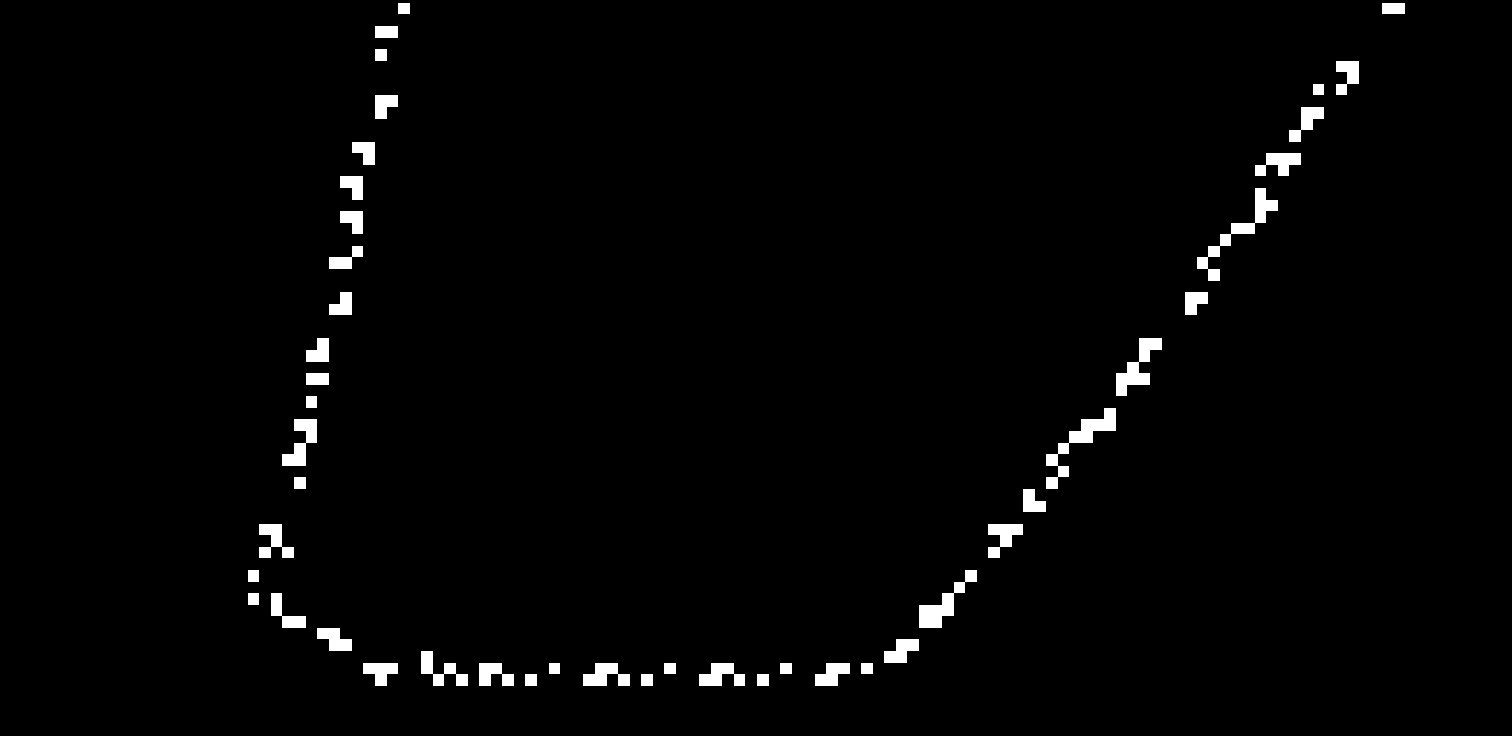
\includegraphics[width=0.90\textwidth]{implemented/failedZeroEx}
\caption{Zero level set corresponding to the label image in figure \ref{labelFailedEx}.}
\label{failedZeroEx}
\end{figure}
The zero level set in figure \ref{failedZeroEx} is the segmentation result (zoomed in) that corresponds to the label image in figure \ref{labelFailedEx}. The zero level set is supposed to be a one pixel wide continous line, but in this case that is not true. Several problems and bugs in the code combined were reasons were for this result. Much time and effort was used to debug this and to fix these problems. In addition to creating artifacts in the results, the bugs also made the program run much slower which made the debugging process even more time consuming. The main problem was that the layers were not of equal range-width and that the speed function was not normalized to be within the range $<\!-1,1\!>$, which will now be explained in more detail.
When an element in any of the five layers is updated by the speed function the new value may not reflect the range at which is allowed for the layer it is part of. In that case it have to be moved to another layer or in case the value is not in the allowed range of any of the layers removed from its current layer and not added to any other. The problem caused by the value returned by the speed function not being normalized was that elements in any layer was able to be transferred from its previous layer to a layer that is not a neihbouring layer. For example, transferring a pixel from Ln1 is restricted to the neighbouring layers of Ln1, namely Ln2 and Lz. But if a pixel $A$ in Ln1 with value -0.65 had its value increased by 1.2, its new value of 0.55 would indicate that it should be moved to Lp1, jumping over Lz. 
As can be seen in table \ref{rangeTab2} all the lists have the exact same range-width of $<1$, which is not the case in table \ref{rangeTab1}. If the ranges in table \ref{rangeTab1} is used it will disort the segmentation process. This happens for example when an element in Lz have the value -0.5 and is increased by 1 by the speed function. A result from the speed functin with value 1 (or -1) indicates fast movement and that element should be moved to Lp1 (or Ln1). But according to table \ref{rangeTab1} that will not happen in Lz when the value is -o.5, even if a change in 1 (or -1) of an element in any other layer would definetly move it out of that layer. But even if an element that should be removed is not removed, an element from either Ln1 or Lp1 is moved into Lz (which is correct behaviour), hence the Lz becomes two pixels wide. An example layer image of this is illustrated in figure \ref{doubleLzLayer}. To clearly illustrate how the double Lz looks like, this figure was sampled after the normalization of the speed function results was implemented.
\begin{figure}[h!]
\centering
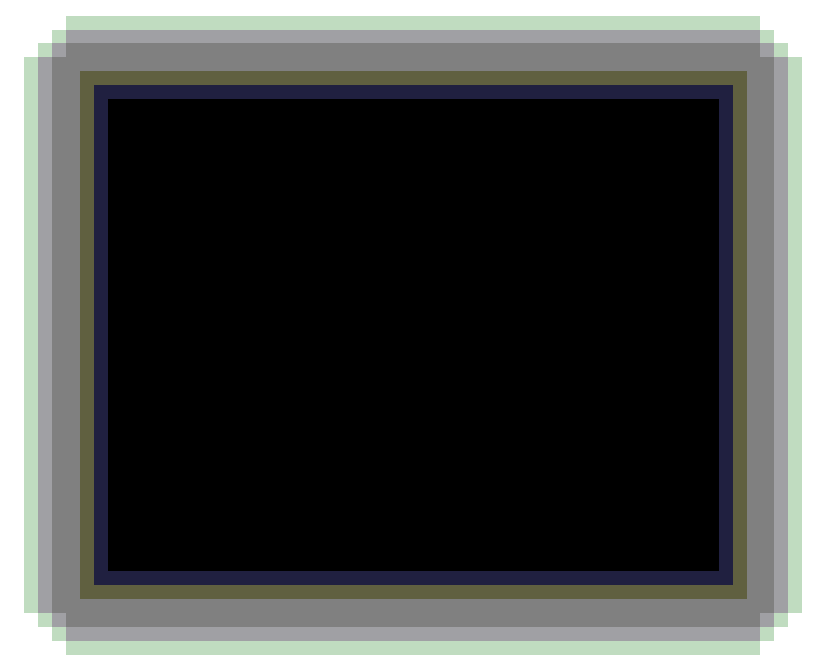
\includegraphics[width=0.80\textwidth]{implemented/doubleLzLayer}
\caption{Layer image with Lz two pixels wide.}
\label{doubleLzLayer}
\end{figure}

Another thing that caused problems was a bug in the code that in some cases moved a pixel from $Lp1$ to $Ln2$ when it was supposed to move to $Lp2$. This bug occured only in the 3D implementation and only under certain circumstances, which made the debugging process more complicated and cumbersome. MER??

\section{CUDA Implementation}
The sparse field level set method was also parallelized by implementing it in CUDA. This process proved to be somewhat more complicated than creating a serial sparse field program. The sparse field method is as mentioned before an optimized version of the narrow band level set method that focuses on using dynamic arrays (linked lists) to hold the elements needed for computation. This is a very serial way of thinking, and parallelization was not a factor when sparse field method was created. 

The most important change in the CUDA implementaion was the addition of another array in the same size as the image to be segmented. This array, called $layer$, is used as an replacement for the five lists and their corresponding temporary lists. This change was made because of two reasons. The first reason is that the only dynamic array structure supported by CUDA (as of May 2013), called thrust and is a C++ template library for CUDA\cite{thrustCuda}, does not support resizing within the device. This is in itself is a reason to not use arrays (dynamic or not) to represent the different layers when the code is structured as it is in the serial versions. The other reason is that the use of an array of same size as the image to be segmented, with each coordinate being handled by a single thread in the GPU utilizes the power of paralleilsm that the GPU provides much better.

The most used method to utilize the parallel capabilities of GPUs when working with 2D and 3D arrays is to split the array in small tiles, each manageable by a CUDA block, and do the processing using the shared memory. This avoids too much use of the slow global memory whic can take hundreds of clock cycles to load data. Comparing this to the 1-2 cycles needed to access data in the local memory a huge difference in speed can be achieved by using the local and shared memory. But doing it this way does however require an almost complete reimplementaion of the code, which due to the limited time was not achievable in this project. Instead an array was used as a whole without splitting it up. 

This is where the $layer$ array mentioned above comes in. This array contains integer values corresponding to each value in the $label$ and $\phi$ arrays. Each element in $layer$ who are member of any of the five layers is represented by a two digit number, and the rest is zero. The first of these two digits is is either 1 or 2. The second digit represents the layer in which that element is a part of, if the digit is 3, 4, 5, 6, or 7 it means that the element is part of Ln2, Ln1, Lz, Lp1 or Lp2 respectively. If the first digit is 2, it corresponds to the element being part of a temporary list. For example, if $label(x,y)$ = $25$ then the element with coordinate $(x,y)$ in the $\phi$ array is part of what in the serial version was called Sz. The decision to make a somewhat unusual array like this was taken to avoid a set of conditional checks in the code, in addition to the resulting consumption of less memory. Using an array like this instead of linked lists makes this implementation close to an extreme narrow band implementation, though the pixel are processed in the way of a sparse field implementation. The only other change from the data-structures used in the serial implementation is the removal of the C++ struct called $Pixel$. This struct only contained the coordinates of elements in any of the five layers, but this is not necassary when not using lists. In the serial version, the calculations of normals and first and second order derivatives were put in a header file, but in the CUDA version these computations were put inside the speed function for performance. The speed function is defined as a \_\_device\_\_ function, which makes it inline with the function calling it. Apart from these changes the CUDA code is very similar to the serial version, hence there is no difference beteween results of full segmentations from the serial and parallelized version.

As described before, the updating process of the layers are dependent on each other. Ln2 and Lp2 are respectively dependent on Ln1 and Lp1, while Ln1 and Lp1 depends on Lz. So even if all the calculations in each element part of the zero level set can be parallelized, all operations in the other layers have to wait. One way to overcome this when in a parallel context is to use barriers to synchronize. But even if all threads within a block are synchronizable using the CUDA defined barrier $\_\_synchthreads()$, there are no native ways to synchronize blocks in CUDA. Some ways to manually synchronize CUDA block exists, for example by using atomic functions to increment a mutex and busy-waiting until the mutex reaches a predefined value or by using lock-free sychronizing as described in \cite{shucai10}. But these methods are only applicable when the number of blocks and threads is smaller than what can be run in parallel (hence no native CUDA block synchronization) which is not the case in this project, where multiple full scale arrays are used. In this case, the only way to achieve the desired feature of ordered execution is to seperate the code into different CUDA kernels. In the serial versions the pseudocode in algorithms \ref{SzAdd}, \ref{Ln12Update} and \ref{Lp12Update} are all executed in the same function, but in the CUDA version the code is split up into several kernel functions. This does affect the performance, but because the global memory is persistent between kernel launches, only slightly. Because only a few neighbouring pixels are elements of the same layers, warp divergence will be affecting the performance more. With the lack of local and shared memory usage, and the bottleneck when accessing the slow global memory results is the implemented CUDA program to use slightly more time to run than the serial version. More abouut the performance will be discussed in chapter REFERANSE TIL ENTEN RESULTS ELLER DISCUSSION HER.

\section{Performance}
Both C++ and Matlab were candidates languuages to implement the level set function in. The adavatage of using Matlab is the simple syntax used for mathematical operations and the ease of loading/writing and displaying images in both 2D and 3D. But ultimately C++ was chosen because of its advantages in speed and the possibility of parallelization. The performance improvements to be discussed in this section was all performed before the implementation of CUDA code. This section will only discuss changes made to improve performance in the serial versions of the code. A comparision of the performance of the serial and CUDA versions of the program will be discussed in chapter LINK TIL ENTEN RESULT ELR DISCUSSION HER.

Several improvements to increase the performance were made after a working 3D version was complete, some which gave insignificant or small performance increases, and a few which greatly improved runtime. One of the changes made to achieve significantly improved runtime was as simple as changing all structures defined as $double$ to $float$. In many cases this change may seem insignificant, but in this case with data structures of sizes as big as $512^3$ and several linked-lists with hundreds of pixels being pushed and popped each itereation, the change reduced the runtime significantly. By changing from using double values which take up 8 byte each, to using float which uses 4 bytes, the memory usage of the array and list structures was reduced by nearly 50\%. A chance that improved the runtime even more significanly was the replacement of the C++ datastructure $std::vector$ with the datastructure $std::list$. When the implementation process started $std::vector$ was chosen as the container for the elements in the different layers, without considering any other candidates. The runtime in 2D using $vwctor$ was not considered slow, hence vector was also used for 3D. But due to the slow speed of the 3D version (when using $vector$) changes were needed. One improvement was the above-mentioned double to float change, and even if this improved performance greatly, more changes that could improve performance were sought after. This resulted in the replacement of the $list$ container with the $vector$ container for the pixels in the different layers. Some of the advantages and disadvantages of using the $std::list$ and $std::vector$ are summarized in table \ref{vectorTab} and \ref{listTab}.

\begin{table}[h!]
	\begin{tabular}{| p{5.85cm} | p{5.85cm} |} 
	\hline
	\multicolumn{2}{|c|}{Vector} \\
	\hline
	Advantages & Disadvantages \\
	\hline
	Insertion/erasure from the end uses constant time. &  Insertion/erasure from other than end is costly (O(n)). \\
	Efficient accessing of its elements. & \\
	\hline
	\end{tabular}
	\caption{Advantages and disadvantages of C++ $std::vector$}
	\label{vectorTab}
\end{table}

\begin{table}[h!]
	\begin{tabular}{| p{5.85cm} | p{5.85cm} |} 
	\hline
	\multicolumn{2}{|c|}{List} \\
	\hline
	Advantages & Disadvantages \\
	\hline
	Fast insertion, extraction and moving of elements in any position. & Consume some extra memory to keep the linking information associated to each element. \\
	 & Cannot access elements by their position. \\
	\hline
	\end{tabular}
	\caption{Advantages and disadvantages of C++ $std::list$}
	\label{listTab}
\end{table}
The reason for the drastical inmprovement in performance when changing from $vector$ to $list$ is the removal of the overhead associated with inserteion and erasure of elements not at the end when using $vector$. After the first few iterations, these two actions happens hundreds of times per iteration, and by changing to $list$ this overhead along with the smaller $log(n)$ overhead when increasing the size of the vector is eliminated. The speedup gained by changing the element types from using double to float and the speedup aquired when replacing $vector$ with $list$ is shown in table \ref{speedUps}.

\begin{table}[h!]
	\begin{tabular}{ c | c | c | c | c |} 
	\cline{2-5}
	 & \multicolumn{2}{|c|}{double $\rightarrow$ float} & \multicolumn{2}{|c|}{vector $\rightarrow$ list}\\
	\cline{2-5}
	 & 100 iteration & full segmentation & 100 iteration & full segmentation  \\
	\hline
	\multicolumn{1}{ |c| } {2D} & TODO & X2 & X3 & X4  \\
	\hline
	\multicolumn{1}{ |c| }{3D} & X1 & X2 & X3 & X4  \\
	\hline
	\end{tabular}
	\caption{Runtime improvements in 2D and 3D.}
	\label{speedUps}
\end{table}

Another change that was considered but later dropped, was to replace the use of $list$ with $std::forward_list$. This structure was considered due to its slightly less overhead when inserting and removing elements which makes it more efficient than $list$. But this improvement in insertion and deletion time over $list$ comes as a consequence of the fact that $forward_list$ is a single linked list, and is thus not able to point to the previous element in the list. The sparse field level set methd can be implemented using single-linked lists instead of double-linked lists, but the implementation in this project depends on the lists being double-linked.

\section{Third party libraries for I/O}
In both 2D and 3D version third party libraries were used to read and write input and output data. In the 2D version a simple open source (under the revised BSD license) C++ library called EasyBMP (\cite{easyBMP}) was used for easily reading and writing Windows bitmap (BMP) image files. In the 3D version the Simple Image Processing Library (SIPL, \cite{sipl} created by the co-supervisor for this project, Erik Smistad is used. SIPL is a C++ library that among other features allows simple load and store of volumes of different types. In addition to volume (and image) processing it supports visualization of the data. In this project SIPL is used for reading and storing medical volume data (can read directly from raw data or using a mhd metafile), and for visualizing the the input volume and the segmentation result for comparision.